%# -*- coding: utf-8-unix -*-
%%==================================================
\tikzset{every picture/.style={line width=0.75pt}} %set default line width to 0.75pt    

\chapter{波动与光学}

\section{参考圆}

简谐振动中,物体的位移$x$满足正弦规律变化\footnote{这里我们不区分所谓的“正弦式变化”、“余弦式变化”,本质上只是后文提及的初相不同而已},即$x = A \sin (\omega t + \varphi)$,其中,$A$被称之为\textbf{振幅},$(\omega t + \varphi)$称之为\textbf{相位}(其随时间而变化),而$t=0$时的相位我们称其为$初相$。

对于一个简谐振动,我们总可以认为其为\textbf{半径为$A$、角速度为$\omega$的匀速圆周运动在$x$轴或者$y$轴上的投影},我们将这个投影后为所需的简谐振动的圆称为\textbf{参考圆}。

\noindent \uline{\textbf{运动学角度理解参考圆}}

如图所示,参考圆上某点在$t$时刻与$x$正方向的角度为$\omega t + \varphi$,其投影为

$$x = A \sin (\omega t + \varphi)$$

可以看出,此投影的运动为简谐运动。
~\\

\noindent \uline{\textbf{动力学角度理解参考圆}}


\section{“同侧法”判断波动方向}

\begin{center}

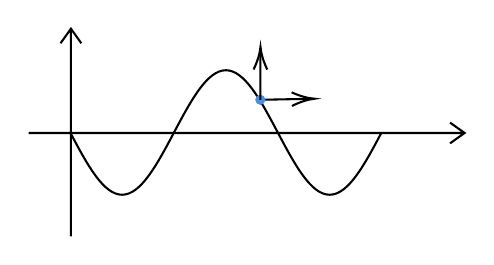
\begin{tikzpicture}[x=0.75pt,y=0.75pt,yscale=-1,xscale=1]
%uncomment if require: \path (0,300); %set diagram left start at 0, and has height of 300

%Shape: Axis 2D [id:dp17044305030121132] 
\draw  (70,150.23) -- (280,150.23)(90.34,100) -- (90.34,200) (273,145.23) -- (280,150.23) -- (273,155.23) (85.34,107) -- (90.34,100) -- (95.34,107)  ;
%Shape: Wave [id:dp3213186683813747] 
\draw   (90,150) .. controls (98.15,165.37) and (105.95,180) .. (115,180) .. controls (124.05,180) and (131.85,165.37) .. (140,150) .. controls (148.15,134.63) and (155.95,120) .. (165,120) .. controls (174.05,120) and (181.85,134.63) .. (190,150) .. controls (198.15,165.37) and (205.95,180) .. (215,180) .. controls (224.05,180) and (231.85,165.37) .. (240,150) ;
%Straight Lines [id:da4960855789495031] 
\draw    (181.58,134.25) -- (205.67,133.77) ;
\draw [shift={(207.67,133.73)}, rotate = 178.86] [color={rgb, 255:red, 0; green, 0; blue, 0 }  ][line width=0.75]    (10.93,-3.29) .. controls (6.95,-1.4) and (3.31,-0.3) .. (0,0) .. controls (3.31,0.3) and (6.95,1.4) .. (10.93,3.29)   ;
%Shape: Circle [id:dp4675822922340589] 
\draw  [color={rgb, 255:red, 74; green, 144; blue, 226 }  ,draw opacity=1 ][fill={rgb, 255:red, 74; green, 144; blue, 226 }  ,fill opacity=1 ] (179.67,134.25) .. controls (179.67,133.19) and (180.52,132.33) .. (181.58,132.33) .. controls (182.64,132.33) and (183.49,133.19) .. (183.49,134.25) .. controls (183.49,135.3) and (182.64,136.16) .. (181.58,136.16) .. controls (180.52,136.16) and (179.67,135.3) .. (179.67,134.25) -- cycle ;
%Straight Lines [id:da7406502193343325] 
\draw    (181.58,134.25) -- (181.66,110.73) ;
\draw [shift={(181.67,108.73)}, rotate = 90.2] [color={rgb, 255:red, 0; green, 0; blue, 0 }  ][line width=0.75]    (10.93,-3.29) .. controls (6.95,-1.4) and (3.31,-0.3) .. (0,0) .. controls (3.31,0.3) and (6.95,1.4) .. (10.93,3.29)   ;

\end{tikzpicture}

\end{center}

一简谐波的波形图($y - x$图)如图所示,上有一质点,判断波的传播方向或该质点此时的运动方向有如下简便的方法。

\begin{theo}{“同侧法”判断波动方向}{}
任取一个\textbf{非顶点}的质点,左右传播方向和该质点运动方向成一个九十度角。如图所示可以用两个剪头分别表示出来。\textbf{在波形图中,这两个箭头一定是在波的同侧出现。}

运用此方法,知道波的振动方向或某时刻质点的运动方向,便可快速判读出另一个方向。

\end{theo}

\section{“旋转法”判断干涉平面凸起还是凹下}

\section{双缝干涉 —— “横乘横等于竖乘竖”}

\begin{center}



\tikzset{every picture/.style={line width=0.75pt}} %set default line width to 0.75pt        

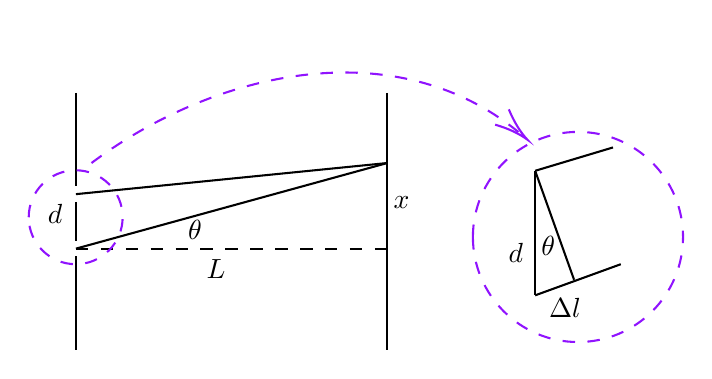
\begin{tikzpicture}[x=0.75pt,y=0.75pt,yscale=-1.5,xscale=1.5]
%uncomment if require: \path (0,300); %set diagram left start at 0, and has height of 300

%Straight Lines [id:da7937139484326525] 
\draw    (130,55) -- (130,85) ;
%Straight Lines [id:da5514747070310864] 
\draw    (130,90) -- (130,102.5) ;
%Straight Lines [id:da3180465848105889] 
\draw    (130,107.5) -- (130,137.5) ;
%Straight Lines [id:da26896276424224896] 
\draw    (230,55) -- (230,137.5) ;
%Straight Lines [id:da7167210011053942] 
\draw  [dash pattern={on 4.5pt off 4.5pt}]  (130,105) -- (230,105) ;
%Straight Lines [id:da7138419970578529] 
\draw    (130,105) -- (230,77.5) ;
%Straight Lines [id:da7800441168755299] 
\draw    (130,87.5) -- (230,77.5) ;
%Shape: Circle [id:dp49969692270722277] 
\draw  [color={rgb, 255:red, 144; green, 19; blue, 254 }  ,draw opacity=1 ][dash pattern={on 4.5pt off 4.5pt}] (114.83,94.92) .. controls (114.83,86.58) and (121.58,79.83) .. (129.92,79.83) .. controls (138.25,79.83) and (145,86.58) .. (145,94.92) .. controls (145,103.25) and (138.25,110) .. (129.92,110) .. controls (121.58,110) and (114.83,103.25) .. (114.83,94.92) -- cycle ;
%Curve Lines [id:da6541923848279152] 
\draw [color={rgb, 255:red, 144; green, 19; blue, 254 }  ,draw opacity=1 ] [dash pattern={on 4.5pt off 4.5pt}]  (135,77.5) .. controls (174.6,47.8) and (233.56,34.36) .. (273.79,68.94) ;
\draw [shift={(275,70)}, rotate = 221.74] [color={rgb, 255:red, 144; green, 19; blue, 254 }  ,draw opacity=1 ][line width=0.75]    (10.93,-3.29) .. controls (6.95,-1.4) and (3.31,-0.3) .. (0,0) .. controls (3.31,0.3) and (6.95,1.4) .. (10.93,3.29)   ;
%Straight Lines [id:da18744774929107222] 
\draw    (277.5,80) -- (302.5,72.5) ;
%Straight Lines [id:da2397390109705031] 
\draw    (277.5,120) -- (305,110) ;
%Straight Lines [id:da21304007677005732] 
\draw    (277.5,80) -- (277.5,120) ;
%Straight Lines [id:da6975177627780123] 
\draw    (277.5,80) -- (290,115) ;
%Shape: Circle [id:dp9982306358023718] 
\draw  [color={rgb, 255:red, 144; green, 19; blue, 254 }  ,draw opacity=1 ][dash pattern={on 4.5pt off 4.5pt}] (257.5,101.25) .. controls (257.5,82.61) and (272.61,67.5) .. (291.25,67.5) .. controls (309.89,67.5) and (325,82.61) .. (325,101.25) .. controls (325,119.89) and (309.89,135) .. (291.25,135) .. controls (272.61,135) and (257.5,119.89) .. (257.5,101.25) -- cycle ;

% Text Node
\draw (171,107.4) node [anchor=north west][inner sep=0.75pt]  [font=\normalsize]  {$L$};
% Text Node
\draw (120,89.9) node [anchor=north west][inner sep=0.75pt]  [font=\normalsize]  {$d$};
% Text Node
\draw (231,87.4) node [anchor=north west][inner sep=0.75pt]  [font=\normalsize]  {$x$};
% Text Node
\draw (268,102.4) node [anchor=north west][inner sep=0.75pt]  [font=\normalsize]  {$d$};
% Text Node
\draw (165,95) node [anchor=north west][inner sep=0.75pt]  [font=\normalsize]  {$\theta $};
% Text Node
\draw (278.5,100) node [anchor=north west][inner sep=0.75pt]  [font=\normalsize]  {$\theta $};
% Text Node
\draw (281,119.9) node [anchor=north west][inner sep=0.75pt]  [font=\normalsize]  {$\Delta l$};


\end{tikzpicture}

\end{center}

如图,一个间距为$d$的双缝,离光屏距离为$L$,干涉条纹间距为$\Delta x$,光的波长为$\lambda$。\textbf{由于光屏比较远(即满足$L \gg d$),则可以近似认为从双缝发出的光到光屏上同一点的光线互相平行}。

记到某一点的两束光光程差为$\Delta l$,第$n$条亮条纹离光屏上的等光程点距离为$x_n$(根据前文近似条件,这里取下面的缝发出光线垂直于光屏时的位置为等光程点\footnote{当然这里也可以取上面的缝对应在光屏上的点或者两缝中点对应在光屏上的点,由于$d$为小量,可以略去不同取法的差别}。)由几何关系,有

$$ \Delta l = d \sin \theta $$
$$ x_n = L \tan \theta $$

由于亮条纹光程差满足$\Delta l = n \lambda$($n \in \mathbb{N^{+}}$),故

\begin{subequations}
\begin{align*}
x_n = L \tan \theta \tikzmarknode{xljs}{\highlight{red}{$\approx L \sin \theta$}} = \frac{L \Delta l}{d} = \frac{n \lambda L}{d}
\end{align*}
\end{subequations}

\begin{tikzpicture}[overlay,remember picture,>=stealth,nodes={align=left,inner ysep=1pt},<-]

\path (xljs.south) ++ (0,-2em) node[anchor=north] (xljsscalep){\highlight{red}{$\theta$为小量时,$\theta \approx \sin \theta \approx \tan \theta$(见“常用小量近似”\eqref{s_xljs})}};
\draw [color=red!87](xljs.south) -- ([color=red]xljsscalep.north);

\end{tikzpicture}

\vspace{2\baselineskip}
因此,两条亮条纹之间间距$\Delta x = x_n - x_{n-1} = \frac{\lambda L}{d}$,故

\begin{theo}{双缝干涉 —— “横乘横等于竖乘竖”}{}
在双缝干涉中,干涉条纹间距$\Delta x$、双缝距离$d$、缝与光屏距离$L$、光的波长$\lambda$满足

$$L \lambda = d \Delta x$$

记忆方法为\textbf{“横乘横等于竖乘竖”}(光为横波,故光的波长记为“横”,乘上“横的距离”(即为$L$,在示意图中它是“横着的”),等于两个“竖的距离”相乘(即为$d$和$\Delta x$,在示意图中它是“竖着的”))
\end{theo}


%\subsection{}
